\chapter{HTTP Interface} \label{chap:HTTPInterface}
In order to allow interaction between a Magentix2 agent and the outside world, an HTTP interface service has been developed. The service is automatically started when the StartMagentix.sh script is executed, so no special action is required. A common use for the HTTP Interface service is a webpage that allows its users to monitor and interact with the agents running in Magentix2. The examples in this section show how to interact with Magentix2 agents using a web page and using Javascript and PHP. However, the use of the HTTP interface is not exclusive for web pages and can be used in other scenarios.
\begin{figure}
	\centering
		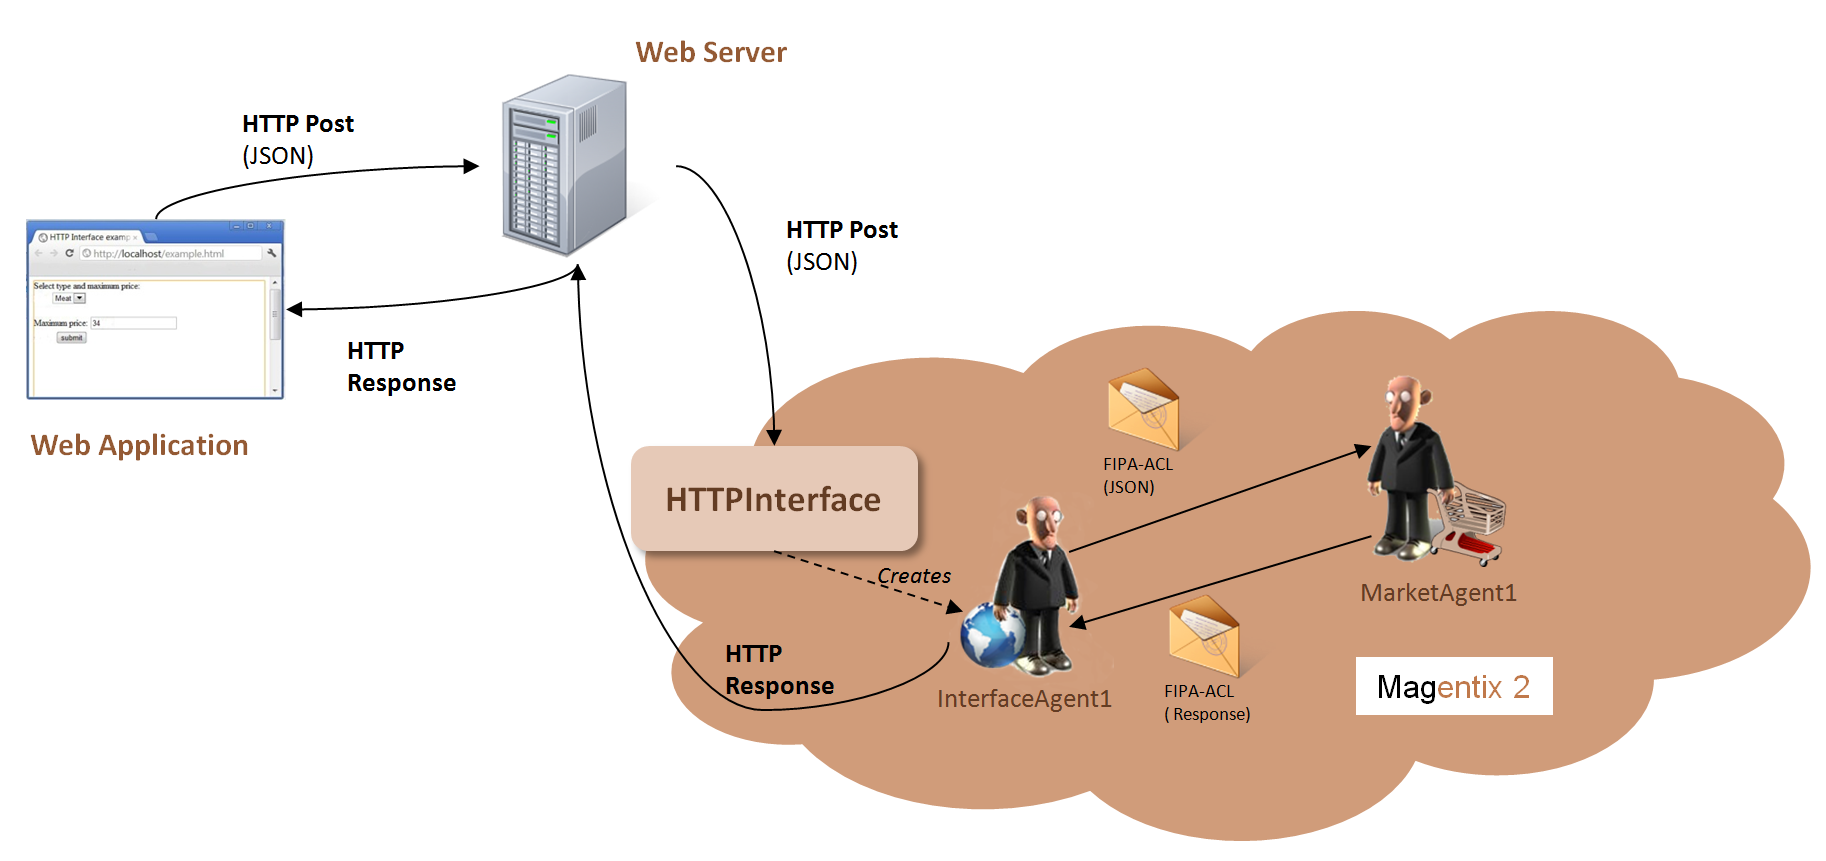
\includegraphics[width=0.95\textwidth]{HTTPInterface/images/HTTPInterface.png}
	\caption{HTTP Interface framewok }
	\label{fig:HTTPInterface}
\end{figure}


\section{Framework}
The functionality of the HTTP Interface service is quite simple. It listens to the port 8081 and expects to get an HTTP POST request. The HTTP interface extracts the target agent from the HTTP POST body message and sends that body message as the content of an ACLMessage to the target agent. 

The information that the HTTP POST request contains must be a well formed JSON\footnote{\url{http://en.wikipedia.org/wiki/JSON}} object. Besides, the JSON object has to obbey to the following guideline:
\begin{itemize}
 \item The JSON object must contain a field called \texttt{agent\_name}. The content of this field is the name of the target agent that will receive the content of the HTTP request.
 \item The object must contain a field called \texttt{conversation\_id}. The content of this field should be a unique identifier. This identifier will be used in the messages sent between the HTTP interface service and the target agent.
 \item The object must also contain a field called \texttt{content}. The content of this field is the information that the target agent will manage.
\end{itemize}

When the HTTP Interface gets the HTTP POST request, it reads the JSON object included in the message body of the HTTP POST request. The HTTP Interface extracts from the JSON object the field \texttt{agent\_name}. The content of this field specifies the target agent. The content of the field \texttt{conversation\_id} of the JSON object will be used as the \texttt{conversation\_id} of the ACLMessage that will be sent to the target message. Finally the entire JSON is used as the content of the ACLMessage. Please note that the entire JSON is used as content, therefore the target agent has to be capable to deal with the fields \texttt{agent\_name} and \texttt{conversation\_id}. Magentix2 includes the XStream library, which is able to manage JSON objects in java. For more information about XStream and JSON, please, go to \url{http://xstream.codehaus.org/json-tutorial.html}. For better understanding, an example of a valid JSON obect is given below. In this example a web page allows users to ask for supermarket products to an agent. The user has to specify the type of the product and the maximum price she is willing to pay.

\begin{lstlisting}
{``agent_name'':``Mike'', ``conversation_id'':``conv1'',``content'':{``type'':``Fruit'', ``max_price'':23.0}}
\end{lstlisting}

The HTTP interface does not send the ACLMessage directly to the target agent, instead, it creates a dummy agent that will send the ACLMessage. This functionality allows the HTTP interface to manage multiple and concurrent HTTP POST requests. The name of a dummy agent is InterfaceAgent\texttt{X}, where \texttt{X} will be a number. As an example, the receiver, conversation\_id, sender and content fields of the ACLMessage that the target agent would recive after the HTTP interface would receive the previous JSON object would be the following:

\begin{lstlisting}
ACLMessage.receiver = Mike
ACLMessage.conversation_id = conv1
ACLMessage.sender = InterfaceAgent1
ACLMessage.content = {``agent_name'':``Mike'', ``conversation_id'':``conv1'',``content'':{``type'':``Fruit'', ``max_price'':23.0}}
\end{lstlisting}

The target agent can respond to the HTTP request sending an ACLMessage to the InterfaceAgent that sent the ACLMessage with the HTTP request. The content of the ACLMessage sent to the InterfaceAgent will be used as the message body of the reply to the HTTP request. Continuing with the previous example, the ACLMessage that the agent Mike would send to the InterfaceAgent1 could be:

\begin{lstlisting}
ACLMessage.receiver = InterfaceAgent1
ACLMessage.conversation_id = conv1
ACLMessage.sender = Mike
ACLMessage.content = {``name'':``Banana'', ``id'':123, ``price'':21.0, }}
\end{lstlisting}

As you may note, the content of this message is a JSON object but it does not follow the guideline explained previously. This is not a problem, the reply content is free and may contain any type of data.

\section{Tools}
Magentix2 provides two tools to facilitate the communication between Magentix2 agents and a webpage: \textit{Magentix2.js} and \textit{Redirect.php} . This tools can be obtained from the examples folder of the Magentix2 distribution. 

\subsection{Magentix2.js}
Magentix2.js is a Javascript library that facilitates the creation of JSON objects that are accepted by the HTTP interface. The two main functions of the library are createJSONObject(agent\_name, conversation\_id, content) and createJSONObject(agent\_name, content). The first one returns a JSON object with the conversation\_id field set to the value passed as parameter. The second one returns a JSON object with a new conversation\_id, this id is a UUID\footnote{\url{http://en.wikipedia.org/wiki/Universally_unique_identifier}}. The parameter content has to be an associative array of elements that will be used as the content of the resulting JSON object.

\subsection{Redirect.php}
This php can redirect an HTTP POST request to any address. You can use it to redirect HTTP POST requests to your HTTP interface. This php requires the Pear HTTP\_Request2 library, you can get this library from \url{http://pear.php.net/package/HTTP_Request2/redirected}.

\section{Example}
In this section only a brief explanation of how to interact with a Magentix2 agent from a webpage is shown. For the complete example, please, refer to the folder examples/httpinterface of your Magentix2 distribution.

The example is composed by two parts:
\begin{itemize}
   \item example.html: This web page contains a form. The user specifies a type of product and a maximum prize. The user will get a product that satisfies her specifications.
   \item MarketAgent: This agent receives the request from the web page example.html and returns an appropriate product.% In order to execute this agent, the blabla script file should be executed. 
\end{itemize}

The example.html webpage uses several javascript libraries in order to send the HTTP POST request asynchronously. These libraries are included in the head section of the html code. The html file also uses our javascript library Magentix2.js. When the user submits the form the javascript function transformData is called.

\begin{lstlisting}
 function transformData(){
	var pp=$("#f1").serializeArray();
	var data=createJSONObject("MarketAgent", pp);
	requestAppData(data);
}
\end{lstlisting}

This function takes every input of the form and constructs an associative array with them. Then it calls to the function createJSONObject of the Magentix2.js library. The parameters are ``MarketAgent'' the name of our agent and the array with the content of the form. The resulting JSON object will be something like this:

\begin{lstlisting}
{"agent_name":"MarketAgent","conversation_id":"5a1a2c78-91b2-465c-818f-bd750ea45f4f","content":{"type":"fruit","max_price":"10"}}
\end{lstlisting}

Finally the transformData calls the function requestAppData with the JSON object as parameter. 

\begin{lstlisting}
function requestAppData(data){
	$.post("redirect.php", data, function(result) {alert("Data Loaded: " + JSON.parse(result));}, "json");
}
\end{lstlisting}

This function calls the jquery function post with the following parameters. Redirect.php is the php script that will redirect our HTTP POST to our HTTP interface. Data is the JSON object previously shown. The next parameter is the function that will be executed when we receive the reply to our request, in this case we will show the result. The last parameter is the type of the data. For more information about jquery and the method jquery.post, please refer to \url{http://jquery.com/}.

MarketAgent is a very simple agent, it receives a query from our webpage and sends a product encapsulated in a JSON object. In the following code, the MarketAgent receives the JSON containing the query and transforms it into a Java object.
\begin{lstlisting}
ACLMessage msg = receiveACLMessage();
XStream xstream = new XStream(new JettisonMappedXmlDriver());
xstream.alias("jsonObject", JSONMessage.class);
JSONMessage query = (JSONMessage)xstream.fromXML(msg.getContent());
\end{lstlisting}

Once the JSON object is a Java object it is possible to work easily with it. The MarketAgent does some calculations with the input data and prepares the response. 

\begin{lstlisting}
 XStream xstream2 = new XStream(new JsonHierarchicalStreamDriver() {
   @Override
   public HierarchicalStreamWriter createWriter(Writer writer) {
      return new JsonWriter(writer, JsonWriter.DROP_ROOT_MODE);
   }
});
String result = xstream2.toXML(product);
response.setContent(result);
this.send(response);
\end{lstlisting}

This time the MarketAgent transforms a Java object into a JSON object. As in the previous step it uses the library XStream. Finally we assign the JSON object as the content of the response message.

Before we can test this example it is important to make sure that the example.html file and the redirect.php script are both in the same web server. By security reasons, cross communication between different hosts is forbidden. Besides, we have to specify in redirect.php the address where our HTTP interface service is running. We can indicate the address modifying the following line in redirect.php:

\begin{lstlisting}
$request = new HTTP_Request2('http://localhost:8081', HTTP_Request2::METHOD_POST);
\end{lstlisting}

In this example the HTTP interface is running in the localhost.







